\section{Конструирование программного средства}

В данном разделе дано описание процесса разработки программного средства.


\subsection{Игровая логика}

Обычно при создании компьютерных игры в первую очередь создают игровую логику. В случае игры, разрабатываемой в данном дипломном проекте, необходимо реализовать логику игрового поля, из-за наличия различных игровых режимов выделить общий для всех режимов интерфейс и на основе этого интерфейса реализовать логику компьютерного противника.


\subsubsection{Игровое поле}

Так, как в такой тип игры может играть только два человека одновременно, то, следовательно, можно объявить следующее перечисление для обозначения текущего состояния клетки игрового поля:

\begin{lstlisting}[caption={Перечисление для обозначения клетки поля}]
public enum SquareSymbol
{
    Blank,
    Zero,
    One
}
\end{lstlisting}

В перечислении SquareSymbol также присутствует отдельный символ Blank для обозначения пустой клетки игрового поля.

Для обозначения же отдельной клетки поля на определённой позиции создана следующая структура:

\begin{lstlisting}[caption={Структура для обозначения позиции клетки поля}, label=Listing:Development:SquarePosition]
[Serializable]
public struct SquarePosition3x3 : IEquatable<SquarePosition3x3>
{
    private const int BoardRowLength = GameBoard3x3.BoardRowLength;
    private const int BoardFullLength = GameBoard3x3.BoardFullLength;

    private int _x;
    private int _y;

    public SquarePosition3x3(int packedPosition)
    {
        ...
        _x = packedPosition % BoardRowLength;
        packedPosition = packedPosition / BoardRowLength;
        _y = packedPosition;
    }

    public SquarePosition3x3(int x, int y) { ... }

    public int X => _x;
    public int Y => _y;

    public static implicit operator int(SquarePosition3x3 position) => position._x +  BoardRowLength * position._y;

    public static implicit operator SquarePosition3x3(int packedPosition) => new SquarePosition3x3(packedPosition);

    ...
}
\end{lstlisting}

Структура SquarePosition3x3 создана специально для игрового поля размером три на три клетки, поэтому в ней есть две константы с размерами поля: BoardRowLength и BoardFullLength.

Также из-за того, что игровое поле реализовано в виде одномерного массива символов позиций на поле (как будет показано далее), то для удобства в этой структуре определенно преобразование в тип \lstinline{int} и обратно путём упаковки двухмерной позиции в одномерную и обратно, как показано на листинге выше. Также такое решение было принято в целях обеспечения для компьютерного противника независимости от типа игрового поля и позиций на нём, что будет показано далее

Для трёхмерного игрового поля структура для обозначения позиции клетки поля схожа со структурой из листинга \ref{Listing:Development:SquarePosition}, за тем различием, что она хранит три координаты и также обеспечивает их упаковку в одномерную координату:

\begin{lstlisting}[caption={Пример упаковки и распаковки трёхмерной позиции}]
// Pack
_x = packedPosition % BoardRowLength;

packedPosition = packedPosition / BoardRowLength;
_y = packedPosition % BoardRowLength;

packedPosition = packedPosition / BoardRowLength;
_z = packedPosition;

// Unpack
packedPosition = _x + BoardRowLength *
    (_y + BoardRowLength * _z)
\end{lstlisting}

Для всех видов игровых полей определён следующий минимальный интерфейс:

\begin{lstlisting}[caption={Интерфейс игрового поля}]
public interface IGameBoard
{
    MoveResult Move(SquareSymbol player, int packedPosition);

    void Reset();

    void CopyTo([NotNull] IGameBoard to);
}
\end{lstlisting}

Интерфейс игрового поля IGameBoard определяет методы для хода, сброса игрового поля в начальное состояние и копирования текущего состояния в другое игровое поле (этот метод необходим для реализации компьютерного противника как будет показано далее). Для обеспечения универсальности данного интерфейса для всех игровых режимов в методе Move() используется упакованная позиция на игровом поле, а результат хода можно узнать по возвращаемому методом значением, состоящем в перечислении MoveResult:

\begin{lstlisting}[caption={Перечисление с результатом хода на игровом поле}]
public enum MoveResult
{
    Continue,
    WrongMove,
    PlayerWin,
    Draw
}
\end{lstlisting}

На основе интерфейса IGameBoard созданы классы с основной игровой логикой для различных игровых режимов. Один из таких классов для игрового режима на двухмерном поле представлен на листинге \ref{Listing:Development:GameBoard3x3}:

\begin{lstlisting}[caption={Класс игрового поля три на три клетки}, label=Listing:Development:GameBoard3x3]
public class GameBoard3x3 : IGameBoard
{
    public const int BoardRowLength = 3;
    public const int BoardFullLength = BoardRowLength * BoardRowLength;

    protected readonly SquareSymbol[] _board = new SquareSymbol[BoardFullLength];

    protected int _movesCount;
    protected SquareSymbol? _winner;

    public MoveResult Move(SquareSymbol player, int packedPosition)
    {
        if (player == SquareSymbol.Blank || _winner != null || packedPosition < 0 || packedPosition >= BoardFullLength || _board[packedPosition] != SquareSymbol.Blank)
          return MoveResult.WrongMove;

        _board[packedPosition] = player;

        _movesCount++;
        _winner = GetWinner(packedPosition);

        switch (_winner)
        {
            case SquareSymbol.Blank:
               return MoveResult.Draw;
            case SquareSymbol.Zero:
            case SquareSymbol.One:
                return MoveResult.PlayerWin;
        }

        return MoveResult.Continue;
    }

    public void Reset() { ... }

    public void CopyTo(IGameBoard to) { ... }

    protected SquareSymbol? GetWinner(int packedPosition) { ... }
}
\end{lstlisting}

Класс игрового поля из листинга GameBoard3x3 содержит константы с размерами игрового поля, одномерный массив с состояниями клеток игрового поля и методами интерфейса IGameBoard.

Отдельно стоит отметить метод GetWinner(): этот метод реализует проверку игрового поля на наличие победителя, в целях оптимизации принимает позицию последнего хода для того, чтобы не проверять все возможные выигрышные комбинации и может возвращать значение символа игрока-победителя, значение SquareSymbol.Blank, если ничья или \lstinline{null}, если победитель не определён и игра не закончена.

Код класса трёхмерного игрового поля схож с кодом класса двухмерного игрового поля из-за использования упакованных позиций и одномерного массива с состояниями клеток игрового поля. Разница лишь в том, что различаются константы с размерами игрового поля и метод GetWinner() имеет другую реализацию с учётом особенностей трёхмерного игрового поля.


\subsubsection{Компьютерный противник}

Игру можно рассматривать как дерево возможных будущих игровых состояний. Текущее состояние игры -- корень дерева. В целом этот узел имеет несколько детей, представляющих все возможные шаги, которые мы могли бы сделать. Каждый из этих узлов имеет детей, представляющих состояние игры после каждого хода противника. Эти узлы имеют дочерние элементы, соответствующие возможным вторым перемещениям текущего игрока, и так далее. Листья дерева являются конечными состояниями игры: состояния, где дальнейший ход не может быть сделан, потому что один игрок выиграл, или, возможно, ничья. На самом деле, в общем случае дерево -- это граф, потому что может быть более одного способа добраться до определенного состояния.

Предположим, что мы присваиваем значению положительной бесконечности состояние листа, в котором мы побеждаем, отрицательную бесконечность в состояниях, в которых побеждает оппонент, и нуль, если ничья. Мы определяем функцию, которая может быть применена к состоянию листа, чтобы определить, какое из этих значений является правильным.

Если мы сможем пройти через все дерево игр, мы сможем выяснить, является ли игра выигрышем для текущего игрока, предполагающего идеальную игру: мы присваиваем значение текущему состоянию игры, когда рекурсивно идем по дереву. В узлах листьев мы возвращаем соответствующие значения. В узлах, куда мы двигаемся, мы берем максимальные значения потомков, потому что хотим выбрать лучший ход, в узлах, где движется противник, берем минимальные значений потомков. Это дает нам следующую процедуру псевдокода для минимаксного поиска:

\begin{lstlisting}[caption={Псевдокод алгоритма минимаксного поиска}]
fun minimax(n: node): int =
    if leaf(n) then return evaluate(n)
    if n is a max node
        v := L
        for each child of n
            v' := minimax (child)
            if v' > v, v:= v'
        return v
    if n is a min node
        v := W
        for each child of n
            v' := minimax (child)
            if v' < v, v:= v'
        return v
\end{lstlisting}

Обычно поиск во всём игровом дереве недопустим, потому что существует огромное количество возможных состояний. Решение состоит в том, чтобы выполнять поиск только по указанной глубине. Функция вычисления (эвристическая функция) расширяется, поэтому она возвращает значение между L и W для позиций игры, которые не являются конечными позициями. Для игровых позиций, которые выглядят лучше для текущего игрока, он возвращает большие числа. Когда предел глубины поиска превышен, статический оценщик применяется к узлу, как если бы он был листом.

Разработка эвристической функции -- это искусство: хорошая эвристическая функция должна быть очень быстрой, поскольку она является ограничивающим фактором в том, насколько быстро работает алгоритм поиска. Но она также должна улавливать разумное приближение того, насколько хороша текущая позиция на доске, потому что она фиксирует то, что игрок пытается достичь во время игры. На практике разработчики AI обнаружили, что не всегда следует строить сложную эвристическую функцию, когда такую же информацию можно получить путем поиска на уровень или два глубже в игровом дереве.

Алгоритм альфа-бета отсечения значительно улучшает алгоритм минимаксного поиска, что устраняет необходимость поиска больших частей игрового дерева с применением техники ветвей и границ. Примечательно, что он делает это без какой-либо возможности пропустить лучший ход. Если кто-то уже нашел хороший ход и ищет альтернативы, достаточно одного опровержения, чтобы избежать его. Нет необходимости искать еще более сильные опровержения. Алгоритм поддерживает два значения: альфа и бета. Они представляют собой минимальную оценку, на который рассчитывает максимизирующий игрок, и максимальную оценку, который гарантирован минимизирующему игроку, соответственно. Псевдокод этого алгоритма отображен на листинге \ref{Listing:Development:AlphaBeta}:

\begin{lstlisting}[caption={Псевдокод алгоритма альфа-бета отсечения}, label=Listing:Development:AlphaBeta]
fun minimax(n: node, d: int, min: int, max: int): int =
    if leaf(n) or depth=0 return evaluate(n)
    if n is a max node
        v := min
        for each child of n
            v' := minimax (child,d-1,v,max)
            if v' > v, v:= v'
            if v > max return max
        return v
    if n is a min node
        v := max
        for each child of n
            v' := minimax (child,d-1,min,v)
            if v' < v, v:= v'
            if v < min return min
        return v
\end{lstlisting}

Для реализаци алгоритма и альфа-бета отсечения в создаваемой игре интерфейса IGameBoard недостаточно, поэтому создаётся новый интерфейс, расширяющий возможности интерфейса IGameBoard:

\begin{lstlisting}[caption={Расширенный интерфейс игрового поля}]
public interface ISearchableGameBoard : IGameBoard, IEnumerable<int>
{
    SquareSymbol MaximizingPlayer { get; }

    int FreeSquaresCount { get; }
    bool IsGameOver { get; }

    new PackedPositionsEnumerator GetEnumerator();

    void MoveUnsafe(bool maximizing, int packedPosition);
    void UndoMoveUnsafe(int packedPosition);

    int GetHeuristics(int depth);
}
\end{lstlisting}

Интерфейс ISearchableGameBoard также наследует интерфейс IEnume \linebreak rable<int> для возможности итерации по свободным клеткам игрового поля. Также определяется свойство для определения завершена ли игра и методы для хода и отмены хода. Отдельно стоит отметить функцию GetHeuristics(): она принимает текущую глубину в дереве поиска и возвращает меру <<выгоды>> относительно текущего состояния игрового поля.

Классы, реализующие интерфейс ISearchableGameBoard, наследуют классы, реализующие интерфейс IGameBoard соответственно игровому режиму и реализую свой вариант эвристической функции. Все эвристические функции реализую следующий алгоритм проверки:

\begin{enumerate}[label=\arabic*, itemindent=\parindent + 2.25ex]
  \item По очереди проверяются все возможные последовательности клеток на поле.
  \item Во время проверки одной последовательности определяется, если ли там символы обоих игроков: если есть, то возвращается число 0, а если на этой последовательности есть только символы одного игрока и пустые клетки, то возвращается количество занятых игроком клеток.
  \item С помощью специальной функции, уникально для каждого игрового режима определяется бонус от количество занятых игроком клеток на одной линии и текущей глубины в дереве поиска.
  \item Полученное на предыдущем шаге значение добавляется к суммарному значению эвристической функции.
  \item Все остальные последовательности клеток на поле обрабатываются таким же образом.
  \item Возвращается полученное суммарное значение всех проверок.
\end{enumerate}

Реализацию класса для альфа-бета отсечения а проекте можно увидеть на листинге \ref{Listing:Development:AlphaBetaSearch}:

\begin{lstlisting}[caption={Реализация алгоритма альфа-бета отсечения}, label=Listing:Development:AlphaBetaSearch]
public sealed class AlphaBetaSearch
{
    private readonly Random _random = new Random();
    private readonly int _searchDepth;

    public AlphaBetaSearch(int searchDepth)
    {
        ...
        _searchDepth = searchDepth == 0 ? int.MaxValue : searchDepth;
    }

    public async Task<int> SearchBestMoveAsync([NotNull] ISearchableGameBoard board, SquareSymbol player, CancellationToken cancellationToken)
    {
        ...

        return await Task.Factory.StartNew(() => SearchBestMoveInternal(board, player,  cancellationToken), cancellationToken);
    }

    private int SearchBestMoveInternal(ISearchableGameBoard board, SquareSymbol player, CancellationToken cancellationToken)
    {
        var maximizing = player == board.MaximizingPlayer;
        var bestValue = maximizing ? int.MinValue : int.MaxValue;
        var bestPositions = new List<int>(board.FreeSquaresCount);

        foreach (var position in board)
        {
            if (cancellationToken.CanBeCanceled)
                cancellationToken.ThrowIfCancellationRequested();

            board.MoveUnsafe(maximizing, position);

            var value = AlphaBetaSearchInternal(board, int.MinValue, int.MaxValue, _searchDepth - 1, !maximizing, cancellationToken);

            board.UndoMoveUnsafe(position);

            if (maximizing ? value > bestValue : value < bestValue)
            {
                bestValue = value;

                bestPositions.Clear();
                bestPositions.Add(position);
            }
            else if (value == bestValue)
                bestPositions.Add(position);
        }

        return bestPositions[_random.Next(bestPositions.Count)];
    }

    private int AlphaBetaSearchInternal(ISearchableGameBoard board, int alpha, int beta, int depth, bool maximizing, CancellationToken cancellationToken)
    {
        if (depth == 0 || board.IsGameOver)
            return board.GetHeuristics(_searchDepth - depth);

        foreach (var position in board)
        {
            if (cancellationToken.CanBeCanceled)
               cancellationToken.ThrowIfCancellationRequested();

            board.MoveUnsafe(maximizing, position);

            var resultValue = AlphaBetaSearchInternal(board, alpha, beta, depth - 1, !maximizing, cancellationToken);

            board.UndoMoveUnsafe(position);

            if (maximizing)
                alpha = Math.Max(alpha, resultValue);
            else
                beta = Math.Min(beta, resultValue);

            if (alpha >= beta)
                return maximizing ? alpha : beta;
        }

        return maximizing ? alpha : beta;
    }
}
\end{lstlisting}

Класс AlphaBetaSearch в конструкторе принимает максимальную глубину поиска и имеет метод SearchBestMoveAsync() для поиска. Метод Search \linebreak BestMoveAsync() является асинхронным, что отправляет его выполнение в отдельный поток и не позволяет блокировать основной поток выполнения, также он поддерживает отмету поиска если игрок решил выйти в главное меню игры не дождавшись хода компьютерного противника.


\subsection{Система UI}

Для реализации в проекте системы UI было решено использовать концепцию MVC для разделения игровой логики и графического представления. Связующим же звеном в этой системе является интерфейс IScreen:

\pagebreak

\begin{lstlisting}[caption={Интерфейс экрана}]
public interface IScreen
{
    event Action ScreenOpening;
    event Action ScreenOpened;
    event Action ScreenClosing;
    event Action ScreenClosed;

    void OpenScreen();
    void OpenScreen(bool highPriority);
}
\end{lstlisting}

Интерфейс IScreen позволяет управлять системой экранов и также позволяет отслеживать текущее состояние экрана. Базовым же классом, от которого наследуются все другие классы экранов является класс ScreenBase, представленный на листинге в приложении А. Класс ScreenBase реализует интерфейс IScreen а также в связи с тем, что графическое представление и анимации сильно связанны с событиями отдельного экрана, принимает реализацию интерфейса IScreenStateAnimator, который управляет внешним видом и поведением экрана и вызывает различные события жизненного цикла экрана.

Пример использования системы UI в проекте можно увидеть на листинге \ref{Listing:Development:PlayScreen}:

\begin{lstlisting}[caption={Класс экрана меню игры}, label=Listing:Development:PlayScreen]
public sealed class PlayScreen : ScreenBase
{
    private ZenjectSceneLoader _sceneLoader;
    private PreferencesManager _preferences;

    private GameModesBundle _gameModes;
    private DifficultiesBundle _difficulties;

    [Header("Targets")]
    [SerializeField]
    private GameModeScrollSnap _gameModeScrollSnap = null;
    [SerializeField]
    private DifficultyScrollSnap _diffucultyScrollSnap = null;

    [Inject]
    private void OnInject(ZenjectSceneLoader sceneLoader, PreferencesManager preferences, GameModesBundle gameModes, DifficultiesBundle difficulties)
    {
        _sceneLoader = sceneLoader;
        _preferences = preferences;
        _gameModes = gameModes;
        _difficulties = difficulties;
    }

    private void Awake()
    {
        _gameModeScrollSnap.SetGameModes(_gameModes.Where(gameMode => !gameMode.Scene.IsNullOrWhiteSpace()));
        _diffucultyScrollSnap.SetDifficulties(_difficulties);
    }

    protected override void OnScreenOpening()
    {
        _gameModeScrollSnap.SetGameMode(_preferences.GameMode);
        _diffucultyScrollSnap.SetDifficulty(_preferences.Difficulty);
    }

    public void OnGameModeChanged(GameModeInfo gameMode) => _preferences.GameMode = gameMode;

    public void OnDifficultyChanged(DifficultyInfo difficulty) => _preferences.Difficulty = difficulty;

    public void OnPlayClicked()
    {
        _sceneLoader.LoadSceneAsync(_preferences.GameMode.Scene, LoadSceneMode.Single, container => container.BindInstance(_preferences.Difficulty)
            .WhenInjectedInto<AIGamePlayerInstaller>());
    }
}
\end{lstlisting}

Класс PlayScreen управляет меню начала игры с компьютерным противником: он имеет ссылки на списки с игровыми режимами и уровнями сложности, которые инициализирует при запуске приложения, синхронизирует их значение по умолчанию с параметрами игры при открытии экрана и также имеет методы, название которых начинается с букв On...(). Эти методы вызываются элементами интерфейса экрана в ответ на действия пользователя вроде нажатия кнопки или изменения текущего выбранного значения в списке. Внешний вид этого экрана представлен на рисунке \ref{Figure:Development:PlayScreen}.

\begin{figure}[ht]
\centering
	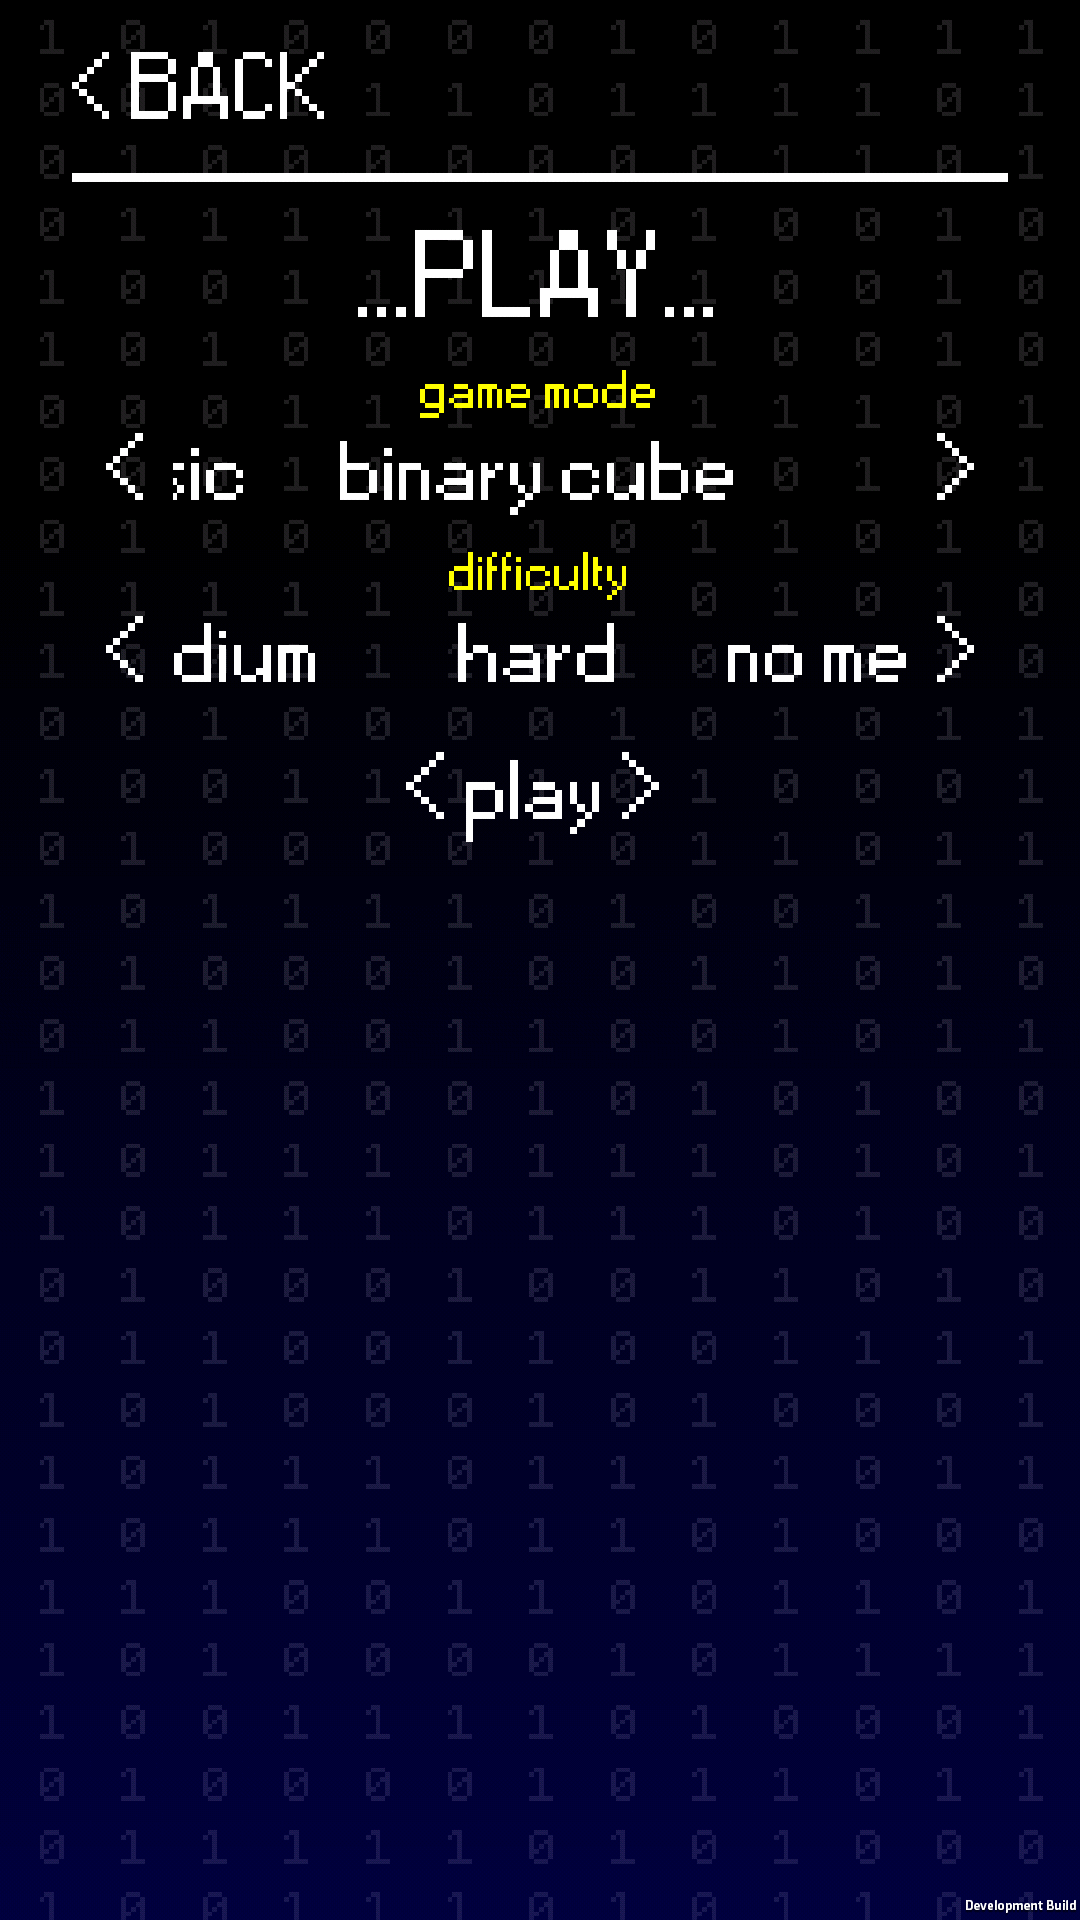
\includegraphics[height=11.5cm, keepaspectratio]{PlayScreen.png}
	\caption{Пример экрана начала игры с компьютерным противником}
	\label{Figure:Development:PlayScreen}
\end{figure}


\subsection{Сетевая система}

Сетевая система в разрабатываемом продукте является авторитарной системой -- вся игровая логика выполняется на стороне сервера, клиент же по сути только получает результаты работы сервера и отправляет ему команды. Сервер обеспечивает синхронизацию состояния игры для всех клиентов. Такая архитектура минимизирует возможность нечестной игры, но требует от сервера обеспечения высокой производительности для лучшей игры. Сетевые возможности разрабатываемого продукта можно подразделить на следующие категории: система организации матчей, менеджер лобби, синхронизация настроек сервера и отдельных игроков, внутриигровой чат, система голосования и ожидания других игроков.

\subsubsection{Система координации игровых сессий}

Система координации игровых сессий призвана облегчить игрокам поиск и создание игровой сессии. Для этого существует отдельный мастер сервер, который контролирует все игровые сессии, клиент же запрашивает у сервера список всех матчей, отправляет запрос на присоединение или создание игровой сессии. Сервер для системы координации игровых сессий предоставляется движком Unity на время разработки на бесплатной основе. От программиста требует только организовать обращение к серверу. Класс MatchMakerManager, осуществляющий эти действия можно увидеть в приложении Б.

Класс MatchMakerManager позволяет создавать сессию, запрашивать список доступных сессий и присоединятся к определённой сессии. Также есть возможность быстрого поиска и присоединения к случайной сессии.

\subsubsection{Менеджер лобби}

Полученная из системы координации игровых сессий информация о сессии используется для присоединения к лобби. Для реализации системы лобби были разработаны классы LobbyManager, LobbyMemberBase, LobbyMember, находящиеся в приложении Б.

Класс LobbyManager является центральным во всей сетевой системе. Он контролирует соединение игроков, работу сетевого сервера и клиента, взаимодействие игроков в лобби и условия начала игры. Также имеет большое количество событий, которые используется по всей игре для контроля и реакции на сетевые события.

Игрокам, состоящим в лобби, требуется наличие способа указания готовности начала игры и синхронизации таких специфичных для игрока настроек, как его имя и используемый им скин. Для этих целей созданы два класса: LobbyMemberBase и LobbyMember.

LobbyMemberBase является абстрактным классом, созданным с для обеспечения игроку в лобби возможности указывания готовности к началу игры и базы для возможности синхронизации параметров игрока между клиентами и сервером. Он имеет виртуальные методы OnClientInitializing, OnClientEnteredLobby, OnClientExitedLobby и OnClientCanJoinChanged, в которых классы-наследники могут организовать начальную установку состояния игрока, также класс предоставляет информацию о готовности игрока к игре и контролирует количество игроков в лобби.

Класс LobbyMember наследует LobbyMemberBase с целью обеспечения синхронизации имени игрока и его скина с сервером и другими игроками. Также он имеет событие ClientInfoChanged, которое вызывается, когда игрок поменял своё состояние и используется для обновления пользовательского интерфейса.

\subsubsection{Чат и синхронизация параметров игры}

Реализация чата состоит из следующих частей: менеджер, отправитель сообщения серверу, отправитель сообщения клиенту и структура для сообщения. Взаимодействие частей происходит следующим образом:
\begin{enumerate}[label=\arabic*, itemindent=\parindent + 2.25ex]
  \item Клиент вызывает у менеджера функцию отправки сообщения.
  \item Менеджер передаёт сообщение клиентскому отправителю сообщений, который вызывает команду отправления сообщения на сервер.
  \item Сервер получает сообщение и пересылает с помощью серверного отправителя сообщений всем клиентам.
  \item Клиенты получают сообщение, добавляют его себе в список сообщений и вызывают событие получения сообщения.
\end{enumerate}

Класс менеджера чата продемонстрирован в приложении В. Менеджер управляет отправлением и получением сообщений, хранит список полученных сообщений и имеет ограничение на их максимальное количество.

Для реализации отправления клиентом сообщения создан класс Chat \linebreak ClientSender, приведённый на листинге \ref{Listing:Development:ChatSender}:

\begin{lstlisting}[caption={Класс отправителя сообщений}, label=Listing:Development:ChatSender]
public sealed class ChatClientSender : NetworkBehaviour
{
    private IChatManagerBackend _chat;
    private IPlayerInfo _playerInfo;

    [Inject]
    private void OnInject(IChatManagerBackend chat) => _chat = chat;

    private void Awake() => _playerInfo = GetComponent<IPlayerInfo>();

    public override void OnStartLocalPlayer() => _chat.RegisterClientSender(this);

    [Client]
    public void ClientSendMessage([NotNull] string message)
    {
        if (message == null)
            throw new ArgumentNullException(nameof(message));
        CmdSendMessage(message);
    }

    [Command]
    private void CmdSendMessage(string message) => _chat.ServerReceiveMessage(_playerInfo.PlayerName, message);
}
\end{lstlisting}

Класс ChatClientSender используется менеджером чата для отправления сообщений. Он присутствует у игрового объекта игрока и получает от него реализацию интерфейса IPlayerInfo для определения имени игрока-отправителя.

Класс ChatServerSender схож с классом ChatClientSender, но организует отправку сообщения с сервера всем клиентам. Его экземпляр создаётся самим менеджером чата во время активации сетевых функций.

Синхронизация параметров сервера с клиентом очень похожа по принципу работы с чатом, но с той разницей, что настройки устанавливаются только на стороне сервера, клиент же не может ничего менять, поэтому нет необходимости в клиентском отправителе. Также вместо хранения списка менеджер настроек хранит только определённые переменные, которые обновляются отдельно друг от друга.


\subsection{Внутриигровой магазин и инвентарь}

Игровой движок Unity уже имеет в своём наличии базовые средства для реализации покупок внутри приложения. Разработчику же необходимо создать слой абстракции для управления внутриигровым магазином как целым.

Для хранения расширенной информации о продуктах и их категоризации созданы два класса, представленные на листингах \ref{Listing:Development:ShopItem} и \ref{Listing:Development:ShopCategory}. Класс ShopItemInfo хранит уникальный идентификатор продукте, его название, тип товара и категорию. Также для хранения дополнительной информации о продукте класс имеет свойство типа Product, которое инициализируется внутриигровым магазином после синхронизации списка купленных продуктов при помощи методов интерфейса IShopItemInitializer. Класс ShopItemCategory служит для разделения продуктов на отдельные категории.

\begin{lstlisting}[caption={Класс продукта}, label=Listing:Development:ShopItem]
[CreateAssetMenu(fileName = "ShopItemInfo", menuName = "Game/Shop/Shop Item Info")]
public sealed class ShopItemInfo : ScriptableObject, IShopItemInitializer
{
    public string Id;
    public string Name;
    public ProductType Type = ProductType.NonConsumable;
    public ShopItemCategory Category;

    public Product Product { get; private set; }
    public bool IsPurchased { get; private set; }

    void IShopItemInitializer.SetProduct(Product product) { ... }
    void IShopItemInitializer.SetIsPurchased(bool isPurchased) { ... }
}
\end{lstlisting}

\begin{lstlisting}[caption={Класс категори продукта}, label=Listing:Development:ShopCategory]
[CreateAssetMenu(fileName = "ShopItemCategory", menuName = "Game/Shop/Shop Item Category")]
public sealed class ShopItemCategory : ScriptableObject
{
    public int Id;
    public string Name;
}
\end{lstlisting}

Для хранения списка продуктов в магазине используется класс Shop \linebreak ItemsBundle, приведённый на листинге \ref{Listing:Development:ShopBundle}:

\begin{lstlisting}[caption={Класс коллекции продуктов}, label=Listing:Development:ShopBundle]
[CreateAssetMenu(fileName = "ShopItemsBundle", menuName = "Game/Shop/Shop Items Bundle")]
public sealed class ShopItemsBundle : ScriptableObject, IEnumerable<ShopItemInfo>
{
    [SerializeField]
    private List<ShopItemInfo> _shopItems = new List<ShopItemInfo>();

    public ShopItemInfo FindById(string shopItemId)
    {
        foreach (var shopItem in _shopItems)
            if (shopItem.Id == shopItemId)
                return shopItem;
        return null;
    }

    ...
}
\end{lstlisting}

На основе представленных выше классов создан класс ShopManager, листинг которого приведён в приложении Г. Данный класс инициализируется коллекцией доступных в магазине товаров, и передаёт его в очередь инициализации. Если инициализация прошла успешно, то объекты продуктов дополняются метаданными о продукте и вызывается событие успешной инициализации. Для начала процесса покупки в классе имеется метод Purchase(), который проверяет, не проводится ли уже покупка в данный момент и передаёт информацию далее магазину целевой платформы. По завершению покупки в зависимости от целевой платформы проводится проверка на достоверность покупки и вызывается событие ProductPurchased, если процесс прошел успешно.

Класс ShopManager используется только для инициализации списка продуктов, осуществления покупки и проверки покупки на достоверность. Для управления же купленными в магазине продуктами используется класс InventoryManager, листинг которого приведён в приложении Г. Класс InventoryManager на основе категории связывает определённые продукты с внутриигровыми предметами и функциями. Так как реализуемому внутриигровому магазину нет необходимости в поддержке большого количества различных категорий товаров, то достаточно лишь поддерживать продукты из категорий <<действия>> и <<скины>>. Прочие классы проекта обращаются к классу инвентаря для получения текущих активированных предметов, и если пользователь хочет активировать внутриигровой предмет в инвентаре, то класс InventoryManager проверяет достоверность покупки и активирует предмет в случае успеха.


\subsection{Аудио система}

Игровой движок Unity уже поддерживает базовые возможности для воспроизведения аудио, но он не имеет средств для организации и управления аудио источниками, также отсутствуют возможности вроде плавного затухания звука, установки очереди проигрывания и т.п.

Для решения этих проблем в создаваемой игры была создана своя аудио система, основанная на группировании различных видов звукового сопровождения и управлении ими как единым целым.

Аудио систему можно представить, как иерархию из следующих компонент:
\begin{itemize}
  \item Глобальный менеджер аудио -- в нём задаются возможные аудио группы и их настройки, обеспечивается их создание и доступ к ним.
  \item Аудио группы -- создаются аудио менеджером с инициализируются настройками, вроде максимального количества аудио источников или громкостью. Создаю и управляют жизненным циклом аудио источников, также обеспечивают проведение операций над подконтрольными аудио источниками в пакетном режим.
  \item Аудио источники -- создаются аудио группами по требованию и обеспечивают воспроизведение одного аудио эффекта за раз. Обладают операциями, схожими с операциями аудио групп, но с тем различием, что они происходят только над текущим аудио источником.
\end{itemize}

Так как в создаваемой игре используются только ограниченное количество аудио групп, то для их идентификации достаточно небольшого перечисления, представленного на листинге \ref{Listing:Development:AudioId}:

\begin{lstlisting}[caption={Перечесление с типами аудио групп}, label=Listing:Development:AudioId]
public enum AudioGroupId
{
    Music,
    SoundFX,
    UI
}
\end{lstlisting}

Для более удобной возможности настраивать существующие аудио группы и из за запрета на возможность менять настройки аудио групп уже после их создания можно создать отдельный класс, представленный на листинге \ref{Listing:Development:AudioConfig}:

\begin{lstlisting}[caption={Класс с настройками аудио группы}, label=Listing:Development:AudioConfig]
[Serializable]
public sealed class AudioGroupConfig
{
    private AudioGroupId _id;

    private int _maxSources;
    private int _preallocatedSources;
    private bool _interruptOldestSourcesForReuse = true;
    private float _volume = 1f;
    private bool _resumeOnUnmute = true;

    private AudioMixerGroup _mixerGroup;

    public AudioGroupId Id => _id;

    public int MaxSources
    {
        get { return _maxSources; }
        private set { _maxSources = value <= -1 ? 0 : value; }
    }

    public int PreallocatedSources
    {
        get { return _preallocatedSources; }
        private set
        {
            if (value <= -1)
                _preallocatedSources = 0;
            else if (_maxSources == 0 || _preallocatedSources <= _maxSources)
                _preallocatedSources = value;
            else
                _preallocatedSources = _maxSources;
        }
    }

    public bool InterruptOldestSourcesForReuse { ... }

    public float Volume
    {
        get { return _volume; }
        private set { _volume = Math.Max(0, Math.Min(1, value)); }
    }

    public bool ResumeOnUnmute { ... }

    public AudioMixerGroup MixerGroup { ... }

    public AudioGroupConfig(AudioGroupId id)
    {
        _id = id;
    }
}
\end{lstlisting}

С помощью класса AudioGroupConfig можно задавать тип группы, максимальное количество звуковых источников, предсоздаваемое количество создаваемых источников, прерывание старых аудио источников при окончании свободных, начальную громкость, автоматическое продолжение воспроизведения аудио после включения звука, аудио микшер.

Класс AudioManager, представленный на листинге \ref{Listing:Development:AudioManager} хранит список с параметрами аудио групп, проводит их проверку, создание и доступ к ним.

\begin{lstlisting}[caption={Класс аудио менеджера}, label=Listing:Development:AudioManager]
public sealed class AudioManager : MonoBehaviour
{
    private readonly Dictionary<int, AudioGroup> _audioGroups = new Dictionary<int, AudioGroup>();
    [SerializeField]
    private List<AudioGroupConfig> _audioGroupsConfigs = new List<AudioGroupConfig>();

    public bool IsInitialized { get; private set; }

    private void OnValidate()
    {
        foreach (var settings in _audioGroupsConfigs)
            settings.Validate();

        foreach (var group in _audioGroupsConfigs.GroupBy(settings => (int) settings.Id))
            Assert.AreEqual(group.Count(), 1,  "Multipy Audio Groups with same Id are found! Audio Groups must have unique Id.");
    }

    private void Awake() => Initialize();

    public IEnumerable<AudioGroup> GetAudioGroups() { ... }

    public AudioGroup GetAudioGroup(AudioGroupId id) { ... }

    private void Initialize()
    {
        if (IsInitialized)
            return;

        foreach (var settings in _audioGroupsConfigs)
        {
            var container = new GameObject($"Audio Group: {settings.Id.ToString().SplitPascalCase()}");
            container.transform.SetParent(transform);

            _audioGroups.Add((int)settings.Id, new AudioGroup(settings, container));
        }

        IsInitialized = true;
    }
}
\end{lstlisting}

Класс AudioGroup, представленный на листинге \ref{Listing:Development:AudioGroup} инициализируется начальными настройками, переданными ему аудио менеджером. Он создаёт и управляет жизненным циклом подконтрольных ему аудио групп, позволяет проводить над ними всеми операции вроде паузы, отключения звука, плавного уменьшения громкости и т.п.

\begin{lstlisting}[caption={Класс аудио группы}, label=Listing:Development:AudioGroup]
public sealed class AudioGroup
{
    private readonly AudioGroupConfig _config;

    private readonly GameObject _audioSourcesContainer;
    private readonly List<AudioSourceAdvanced> _audioSources;

    private float _volume;
    private Tween _volumeFadeTween;
    private bool _mute;

    public AudioGroup([NotNull] AudioGroupConfig config, [NotNull] GameObject audioSourcesContainer) { ... }

    public AudioGroupId Id => _config.Id;
    public bool IsVolumeFading => _volumeFadeTween?.IsPlaying() == true;
    public float Volume { ... }
    public bool Mute { ... }

    public AudioSourceAdvanced Play(AudioClip clip, float volume = 1, float pitch = 1, bool loop = false) => PlayFrom(clip, 0, volume, pitch, loop);

    public AudioSourceAdvanced PlayFrom(AudioClip clip, float fromTime, lume = 1, float pitch = 1, bool loop = false)
    {
        var audioSource = GetAvailableAudioSource();
        if (audioSource != null)
            ResetAudioSource(audioSource).PlayFrom(clip, fromTime, volume, pitch, loop);
        return audioSource;
    }

    public void Resume() { ... }
    public void Pause(){ ... }
    public void Stop() { ... }

    public AudioGroup FadeVolumeInFrom( ... ) { ... }
    public AudioGroup FadeVolumeInTo( ... ) { ... }
    public AudioGroup FadeVolumeOutFrom( ... ) { ... }
    public AudioGroup FadeVolumeOutTo( ... ) { ... }

    public AudioGroup FadeVolume(float from, float to, float duration = .5f, bool ignoreTimeScale = true, Ease ease = Ease.Linear, FadeBehaviour onCompleteBehaviour = FadeBehaviour.None, Action<AudioGroup> onComplete = null) { ... }

    public void OnVolumeFadeComplete(Action<AudioGroup> onComplete) { ... }

    private AudioSourceAdvanced GetAvailableAudioSource() { ... }
    private AudioSourceAdvanced CreateAudioSource() { ... }
    private AudioSourceAdvanced FindOldestAudioSource() { ... }}
}
\end{lstlisting}

Класс аудио источника внешне похож на класс аудио группы, но с тем различием, что он отвечает за воспроизведение только одного звукового эффекта за раз и позволяет установить действие, происходящее по окончанию проигрывания текущего звукового эффекта, как показано на листинге \ref{Listing:Development:AudioExample}:

\begin{lstlisting}[caption={Пример использования аудио системы}, label=Listing:Development:AudioExample]
_musicAudioGroup.Play(_preWinClip).OnPlaybackComplete(source => source.Play(_winClip, loop: true));

_musicAudioGroup.FadeVolumeOutFrom(onComplete: group => group.FadeVolumeInTo().Play(_battleClip, loop: true));
\end{lstlisting}